
\chapter{Implementation Details} \label{chapter:methods}

% Introduction
Chapter \ref{chapter:exp-setup} established the experimental framework for this work.
Then, Chapter \ref{chapter:models-used} detailed the two \acrshort{fspm}s we selected for our experiments.
In this chapter, we explain how we implemented the experiments.
We discuss the adaptations that we made to the simulations, how we handled data for the regression tasks, and how we implemented the impulse experiment.


\section{Preparing the Simulations}

We used the same environmental inputs as the models' original publications for all experiments because the authors only verified the models for these climate conditions.
The complete hourly data for HydroShoot and CN-Wheat can be found in \mbox{Appendix \ref{app:meteo}}.
HydroShoot required small adaptations to the soil water model because empirical soil water data was only available for four consecutive dates. 
We ran CN-Wheat simulations with no modifications.
Details for reproducing the exact simulation setup for both models, as well as descriptions of model modifications we made can be found in Appendices \ref{app:hydroshoot-sim-details} and \ref{app:cnwheat-simulation}.


\section{Observing The Plant Model}

We extracted time series for all physiological processes listed in \mbox{Table \ref{table:simulation_reservoirs}} from each structural element of the \acrshort{fspm}.
The reservoirs are then constructed from this data.
This work investigates homogeneous reservoirs only; we only considered the spatial variations of a single process, not the dynamics between two or more processes. 
However, some preliminary work with heterogeneous reservoirs showed promising results, which can be explored in further research.

It is impossible to get exact measurements or observe the entire plant at once in a real-world scenario.
To make our results more representative for follow-up research, we decided only to observe a fraction of the plant's structure to limit the observability of the reservoir.
We used a reservoir sample size of 32 for HydroShoot and 7 for CN-Wheat. 
This corresponds with approximately \SI{10}{\percent} and \SI{70}{\percent} of the total structure, respectively.
We chose 32 for HydroShoot to limit the number of readout parameters and because we observed that the reservoir performance showed negligible improvements for larger sample sizes.
We only had ten structural elements to observe the chosen physiological processes in CN-Wheat. 
We selected a sample size of 7 to avoid the total observability of the reservoir.
Observing the entire reservoir may introduce bias as the plant model uses the same observations to compute the physiological tasks.
Appendices \ref{app:hydroshoot-reservoir} and \ref{app:cnwheat-reservoir} further elaborate on how the reservoir was constructed for HydroShoot and CN-Wheat, respectively.

% TODO (OPTIONAL): Add figma illustration showing a sketch of a plant, then zoom in on one structural element, then zoom in on the series extracted from it.

\section{Data Preprocessing} \label{sec:data-preprocessing}

First, the raw simulation outputs are combined into a single dataset. Appendices \ref{app:hydroshoot-dataset} and \ref{app:cnwheat-dataset} explain how we did this for each model specifically.
Once we have a single dataset, some preprocessing steps are applied.
Next, we discarded data from the first four days of each simulation run to avoid transient dynamics present during model warm-up.
We also discarded 8 hours of nighttime from each day, between 22:00 and 4:00.
% The considered physiological processes fall idle during these hours.
By discarding these samples from the dataset, we focus the model's capacity on predicting the more detailed and intricate daytime dynamics instead of concentrating on the broader day/night dynamic.
Figure \ref{fig:preprocessing-train-test-split} illustrates the data that is discarded.

Finally, we rescaled both the target and the reservoir series to have zero mean and unit variance.
When we scaled each dimension independently, we noticed a drop in model performance.
We hypothesize that this is due to lost information about the relative difference between observed elements.
Because the observations of the reservoir elements are not independent of each other, we instead rescaled the reservoir using the mean and variance of the reservoir as a whole.

\section{Train and Test Data Split} \label{sec:train-test-split}

To avoid bias in the model scores, we require a set of unseen test data to validate the performance of the final model.
Therefore the optimal model parameters should be trained using only a subset of the total dataset.
We used a train-to-test ratio of 0.5 for all our regression experiments.
Figure \ref{fig:preprocessing-train-test-split} shows how we divided the data samples into train and test sets.
Time series data naturally shows a high degree of temporal correlation.
To reduce the surface area for information leaking between train and test sets, we divided the data into blocks of four days.
The previously mentioned process of discarding the nighttime samples further limits the information leakage between adjacent blocks of train and test data.
% Because the samples from the same day are highly temporally correlated, we grouped the data in blocks of 24 hours that should stay together.
% We then assign the groups to the train or test set in alternating blocks of 4 days.
% This further decreases the information leakage between training and testing data.

\begin{figure}[ht]
	\centering
    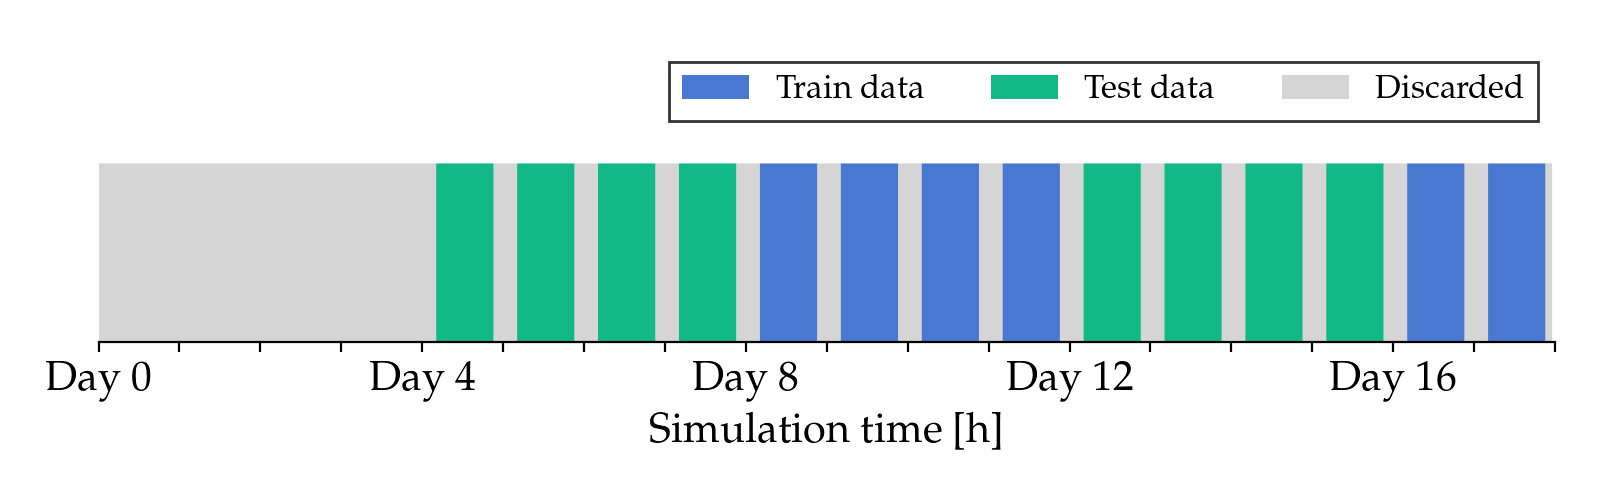
\includegraphics[width=13.33cm]{img/preprocessing_traintestsplit.png}
	\caption[Illustration of the data that is discarded as a preprocessing step and how the remaining data is split into a train and test set.]{Illustration of the data that is discarded as a preprocessing step and how the remaining data is split into a train and test set.}
	\label{fig:preprocessing-train-test-split}
\end{figure}

\section{Model Validation} \label{methods:validation}

The model parameters for each reservoir-target pairing are fitted using ridge regression (\mbox{Equation \ref{esn:training}}).
To find the optimal regularization parameter $\lambda$, we performed a parameter sweep from 0.0001 to 100 with fifty logarithmically spaced values.
We validated the choice of $\lambda$ using the cross-validation method.
In this scheme, the training data is split into ``folds'' of roughly equal size. 
The model is trained using data from all but one fold.
The final fold is used to validate the model, using the \acrshort{nmse} metric.
We repeat this until we have used all folds as validation data.
The mean \acrshort{nmse} across all validation folds suggests the model performance for that value of $\lambda$.
We pick the value of $\lambda$ that yields the best mean validation score.
Once the optimal $\lambda$ is selected, we train a final model using all available training data.

Figure \ref{fig:methods-cv-folds} shows how we created our cross-validation folds. 
We group the folds per calendar day to avoid putting data from the same simulation day in both the train and validation sets.
Otherwise, we risk introducing bias in the validation score thanks to the high temporal correlation between samples of the same input day.
We used the leave-one-group-out strategy, which means we used only one day of data for validation in each iteration.
See Appendices \ref{app:hydroshoot-validation} and \ref{app:cnwheat-validation} for plant information specific to the HydroShoot and CN-Wheat datasets.
% Groups of data samples from the same input day stay together; otherwise, we leak highly correlated data between the train and validation data.

\begin{figure}[ht]
	\centering
    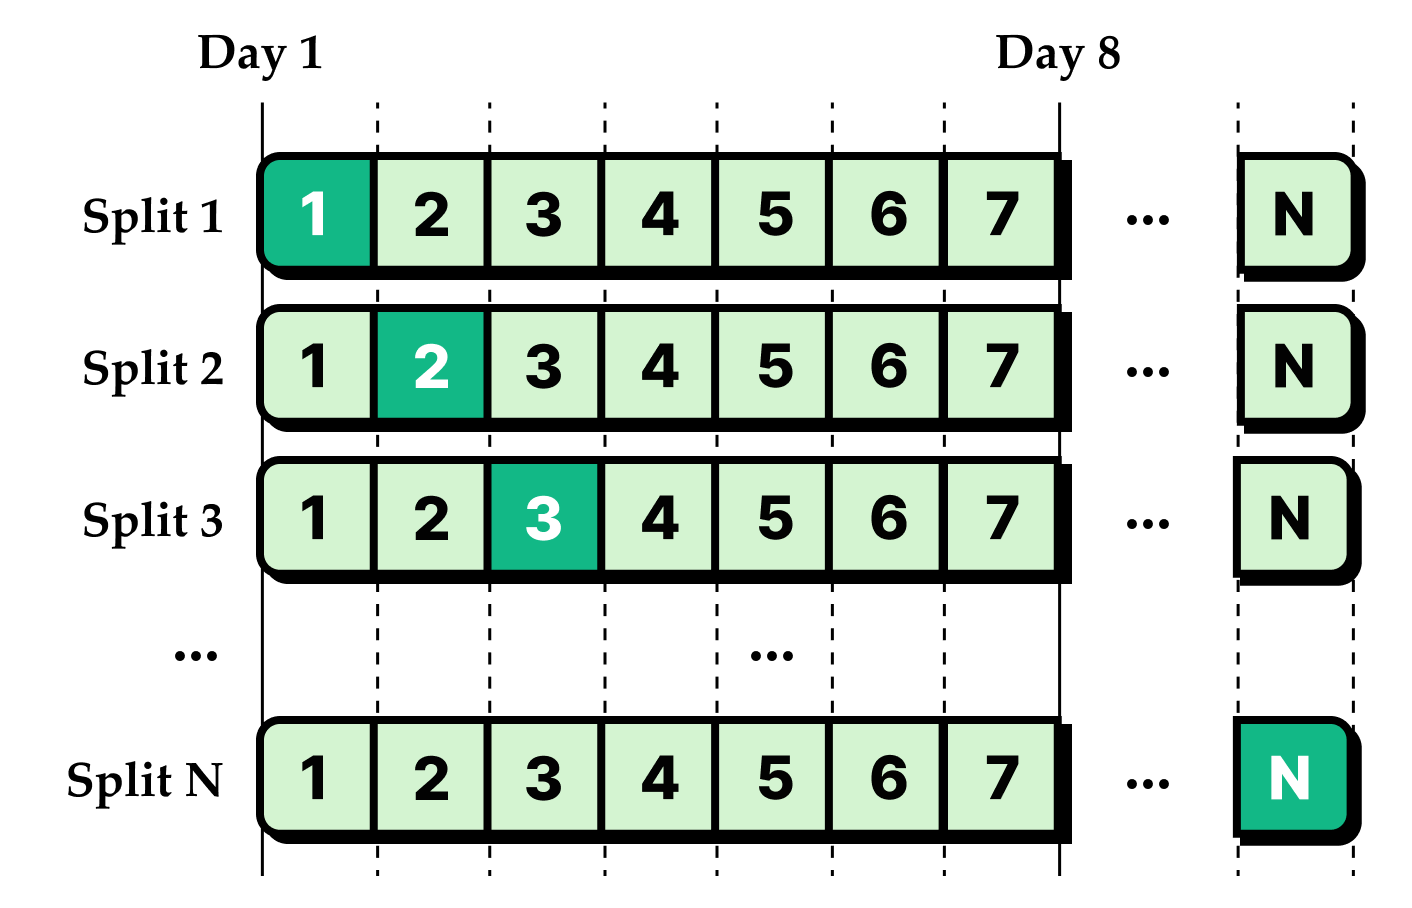
\includegraphics[width=10.5cm]{img/cv-folds.png}
	\caption[Illustration of leave-one-group-out cross-validation strategy.]{Leave-one-group-out cross-validation strategy. Each block represents samples generated from the same calendar day of meteorological inputs. In each split, the highlighted data is used as validation data, the other folds are used for training.}
	\label{fig:methods-cv-folds}
\end{figure}


\section{Implementing the Impulse Experiment}

To implement the impulse experiment, we modified the meteorological input data before running the simulations.
Figure \ref{fig:methods-impulse} demonstrates how the impulse is added to an environmental signal.
The stimulus was applied at least four days after the simulation started to account for transient warmup dynamics in the plant model.
We chose four days because this is the same as the warmup period we assumed in \mbox{Section \ref{sec:data-preprocessing}}.
The model is allowed to run at least five more days after the impulse to capture the fading memory effect completely.
The impulse is always centered on midday and is applied instantaneously.
Appendices \ref{app:hydroshoot-impulse} and \ref{app:cnwheat-impulse} disclose the exact simulation configuration for HydroShoot and CN-Wheat respectively.

\begin{figure}[]
	\centering
    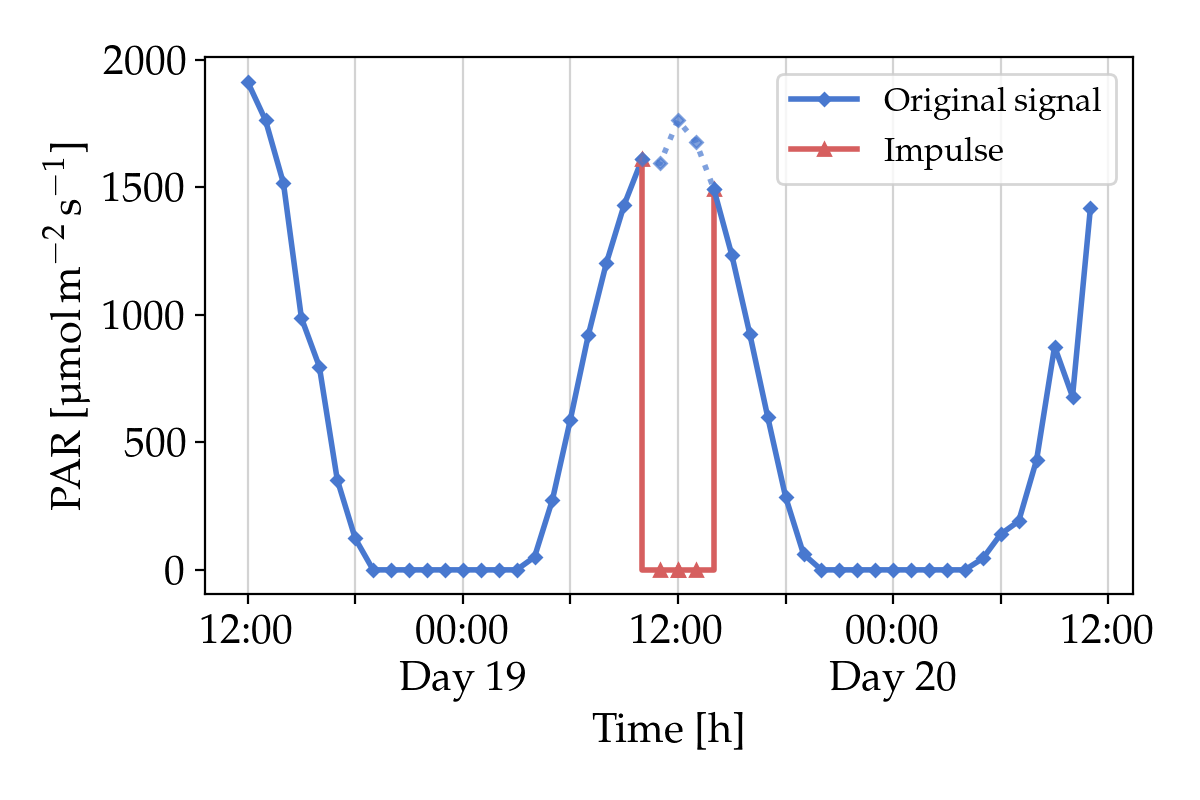
\includegraphics[width=10cm]{img/cn_impulse.png}
	\caption[Adding an artificial impulse to an environmental input.]{Adding an artificial impulse to an environmental input. In this figure we applied an impulse with a width of three hours and a value of \SI{0}{\micro\mole\per\square\meter\per\second} to the incident \acrshort{par} of CN-Wheat.}
	\label{fig:methods-impulse}
\end{figure}

\section{Summary}

This chapter disclosed the implementation details required to reproduce the experimental results presented in this work.
We discussed how the reservoir dataset is constructed, what data preprocessing is applied, how a test dataset is created, and we how validated the readout model parameters. 
We also documented how we implemented the impulse experiment.
We reported additional information on how HydroShoot and CN-Wheat were used in Appendices \ref{app:hydroshoot} and \ref{app:cnwheat}.
